\sect{System Architecture}

\subsect{Tree Parameters}

In order to reap the full benefit of the tree data structure, an informed choice
of parameters must be made that takes consideration of the expected workload and
usage of scarce memory resources.

The tree's branching factor $m$ defines the maximum number of children that each
node can have. A level $k$ down the tree from the root will contain $m^k$ nodes.
Thus, a tree of height $h$ will contain
$\sum_{k=1}^h m^k = \frac{1-m^h}{1-m}$ nodes.

The ratio of leaf nodes to internal nodes is given by:
$$
	\frac{m^{h-1}}{\pfrac{1-m^{h-1}}{1-m}}
	= \frac{m^{h-1}(1-m)}{1-m^{h-1}}
	= \frac{m^{h-1}-m^{h}}{1-m^{h-1}}
	% = \frac{m^h-m^{h+1}}{m-m^h}
	% = \frac{m^h(1-m)}{m^h(m^{1-h} - 1)}
	= \frac{1-m}{m^{1-h} - 1}
$$

As $h$ increases, this rapidly converges to $m-1$ as shown in
\autoref{fig:inner-to-height}.

\begin{figure}
	\centering
	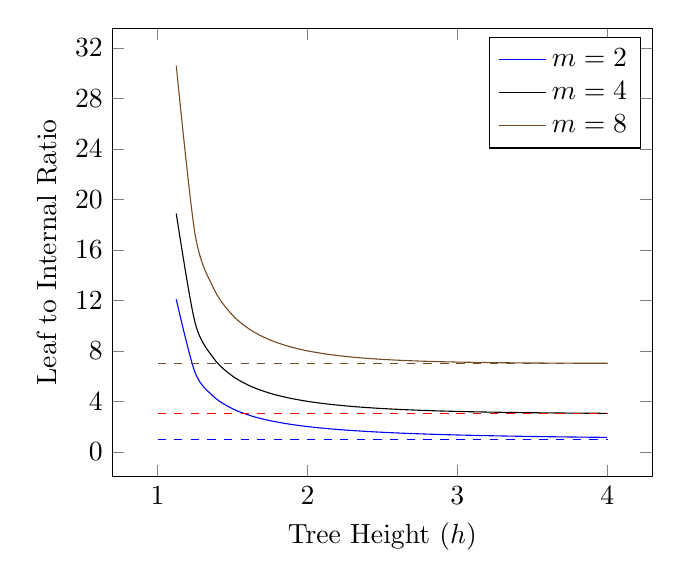
\begin{tikzpicture}
	\begin{axis}
		[
			xlabel={Tree Height ($h$)},
			ylabel={Leaf to Internal Ratio},
			xtick distance=1,
			ytick distance=4,
			domain=1:4,
			smooth
		]
		\pgfplotsinvokeforeach{2,4,8} {
			\addplot+[cycle list name=color list, mark=none]
				{(1-#1) / (#1^(1-x) - 1)};
			\addlegendentry{$m=#1$}
		}
		\pgfplotsset{cycle list shift=-3};
		\pgfplotsinvokeforeach{2,4,8} {
			\addplot+[cycle list name=color list, mark=none, dashed] {#1-1};
		}
	\end{axis}
\end{tikzpicture}

	\caption{Leaf to Inner Node Ratio vs Height}
	\label{fig:inner-to-height}
\end{figure}

As the height of a tree grows, the portion of overall memory that is used for
leaves decreases, converging to $1-\frac{1}{m}$ as shown in
\autoref{fig:memory-to-height}. Higher branching factors spend less memory on
traversal data. Recall that internal nodes do not store data; they store
pointers to other nodes to accelerate lookups over a flat ordered list. Such a
flat list of $n$ elements is equivalent to a B-Link tree of $m=n$ and $h=1$.

\begin{figure}
	\centering
	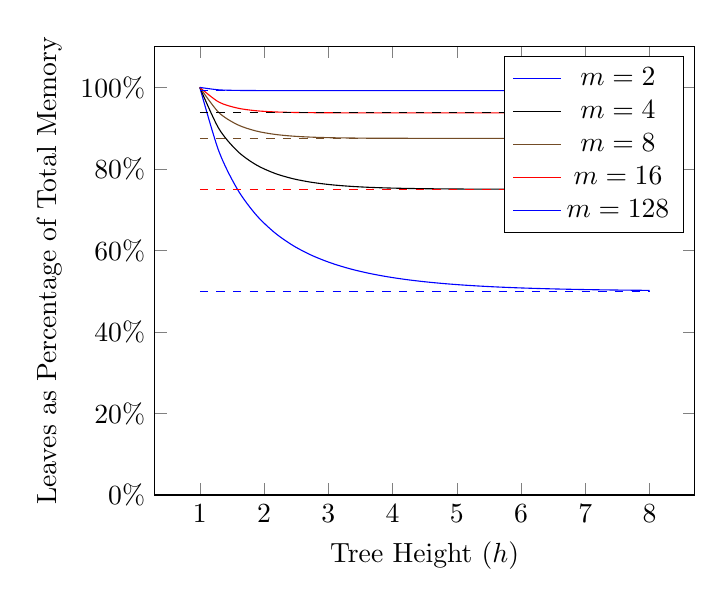
\begin{tikzpicture}
	\begin{axis}
		[
			xlabel={Tree Height ($h$)},
			ylabel={Leaves as Percentage of Total Memory},
			xtick distance=1,
			yticklabel={%
				\pgfmathparse{\tick*100}%
				\pgfmathprintnumber{\pgfmathresult}%
				\%%
			},
			domain=1:8,
			ymin=0,
			smooth
		]
		\pgfplotsinvokeforeach{2,4,8,16,128} {
			\addplot+[cycle list name=color list, mark=none]
				{#1^(x-1) / ((1-#1^x)/(1-#1))};
			\addlegendentry{$m=#1$}
		}
		\pgfplotsset{cycle list shift=-5}
		\pgfplotsinvokeforeach{2,4,8,16,128} {
			\addplot+[cycle list name=color list, mark=none, dashed]
				{1-(1/#1)};
		}
	\end{axis}
\end{tikzpicture}

	\caption{Leaves as Percentage of Total Memory vs Height}
	\label{fig:memory-to-height}
\end{figure}

A tree containing $N$ nodes will have the height shown below.

\begin{align*}
	N &= \frac{1-m^h}{1-m} \\
	N (1-m) &= 1-m^h \\
	N (1-m) - 1 &= -m^h \\
	1 - N (1-m) &= m^h \\
	\log_m\left(1 - N (1-m)\right) &= h
\end{align*}

As $N$ grows, this relation can be approximated as $h \approx 1 + \log_m(N)$,
which is equivalent to  $m^{h-1} \approx N$. Because $m^{h-1}$ is the number of
leaf nodes, this expression approximates the total count of nodes as the number
of leaf nodes. As follows from previous derivations and shown in
\autoref{fig:nodes-to-height}, this approximation is more accurate for larger $m$
where there are more leaves per inner node.

\begin{figure}
	\centering
	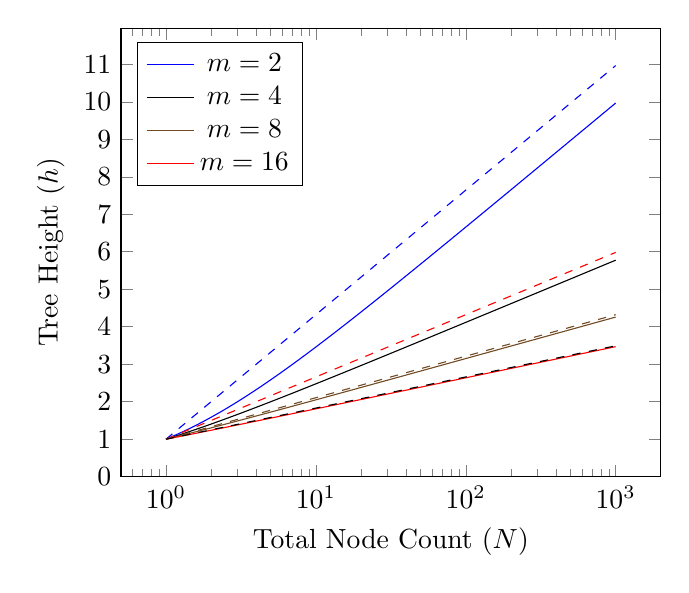
\begin{tikzpicture}
	\begin{axis}
		[
			xlabel={Total Node Count ($N$)},
			ylabel={Tree Height ($h$)},
			domain=1:1000,
			xmode=log,
			ytick distance=1,
			legend pos=north west,
			smooth
		]
		\pgfplotsinvokeforeach{2,4,8,16} {
			\addplot+[cycle list name=color list, mark=none]
				{ln(1 - x*(1-#1)) / ln(#1)};
			\addlegendentry{$m=#1$}
		}
		\pgfplotsset{cycle list shift=-4}
		\pgfplotsinvokeforeach{2,4,8,16} {
			\addplot+[cycle list name=color list, mark=none, dashed]
				{1+ln(x)/ln(#1)};
		}
	\end{axis}
\end{tikzpicture}

	\caption{Height vs Node Count}
	\label{fig:nodes-to-height}
\end{figure}


\subsect{Concurrency}

Our design is based on that of \citeauthor{base} in \citetitle{base}. Their
design uses a CPU cluster with an RDMA interconnect. The design follows the
Network-Attached-Memory (NAM) architecture, where some nodes are dedicated to
computation while others are dedicated to storage
\autocite{base,binnig-vldb-2016}.

To support concurrent access, their design uses optimistic lock coupling rather
than traditional lock coupling. This strategy does not protect areas from
concurrent access, but simply identifies when data has been changed. If two
writers begin modifying the same data, the one who writes back to main memory
second will see that its version is not what was expected, and attempt to
restart its operation using this new data. A key advantage of this strategy is
reducing cache misses due to cache invalidations that result when frequently
writing to lock bits in main memory on multi-core CPUs
\autocite{leis-damon-2016}. On an FPGA, we have the freedom to design our own
caching protocol rather than mimic the general purpose caching protocols that
are fixed in the silicon of CPUs. Thus, this problem could be negated by
managing lock bits differently from other memory to reduce caching overhead
rather than avoiding writes altogether. As noted by
\citeauthor{binnig-vldb-2016}, DBMSs function best with full control over memory
management \autocite{binnig-vldb-2016}.


\subsect{Memory Layout}

Even without the considerations of caching that would arise on CPU-based
systems, memory access patterns can still have significant performance impacts.
The XCU280 FPGA integrates $\SI{8}{\giga\byte}$ of on-chip High-Bandwidth Memory
(HBM) with a theoretical maximum bandwidth of $\SI{460}{\giga\byte\per\second}$
\autocite{u280}, but this is contingent on spreading out the accesses across all
available channels \autocite{holzinger-ipdpsw-2021}.

Though using HLS prevents some of the lower-level access optimizations proposed
by \citeauthor{holzinger-ipdpsw-2021}, it is still possible to reap some
benefits by controlling memory access patterns. Because the manner that the
abstract tree is accessed is dictated by \citeauthor{b-link}'s original
algorithm, the best way to optimize memory accesses is to consider how best to
lay out the tree in memory.

\begin{figure}
	\centering
	\begin{tikzpicture}[
		tree/.style={draw,circle,inner sep=0.25mm,minimum size=14pt}
	]
	\node[tree] at (0, 0) (00) {$0,0$};
	\foreach \r [
		evaluate = \r as \w using int(3^\r),
		evaluate = \r as \wl using int(3^\r-1)
	] in {1,...,2} {
		% Columns
		\foreach \c [
			evaluate = \c as \i using int((\w-1)/2 + \c),
			evaluate = \c as \pr using int(\r-1),
			evaluate = \c as \pc using int(\c/3),
		] in {0,...,\wl} {
			\node[tree] (\r\c)
				at ({0.7*\c}, -\r) {$\r,\c$};
			\draw[-] (\pr\pc.south)
				-- ++(0, {-((3-\pc) + (\pr-1))/9}) -| (\r\c);
		}
	}
	\node[anchor=east] (legend) at (00 -| 28) {Node text is $r,c$};
	\node[anchor=east, below=0.1 of legend] {$m=3, h=3$};
\end{tikzpicture}

	\caption{Rectangular Grid Layout}
	\label{fig:grid-layout}
\end{figure}

Two memory layout schemes have been implemented. The first maps the tree to a
simple rectangular matrix as shown in \autoref{fig:grid-layout}. Each row of the
matrix corresponds to nodes at the same same level of the tree. Note that these
are not all inherently siblings of one another, as leaf nodes with different
parents are still at the leaf-node level of the tree. This strategy maintains
locality for tree levels and allows for easy determination of what level a node
resides in, but wastes more memory the closer a level is to the root.

This strategy also imposes a stricter height limit on the tree than may be
possible with a given amount of memory. Though B-trees are considered
``self-balancing'' in the academic sense due to their limits on underfull nodes,
there is no guarantee of a constant height for all sub-trees. The easiest
demonstration of this is to observe the insertion of a sequence of monotonically
increasing keys shown in \autoref{fig:sequential-imbalance}.

\begin{figure}
	\centering
	\begin{subfigure}{5em}
	\centering
	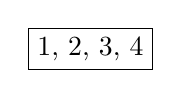
\begin{tikzpicture}
		\node[draw] (root) {1, 2, 3, 4};
	\end{tikzpicture}
	\caption*{One Node}
\end{subfigure}
\begin{subfigure}{7em}
	\centering
	\begin{tikzpicture}[node distance=0.25]
		\node[draw] (leaf1) {1, 2};
		\node[draw] (leaf2) [right=of leaf1] {3, 4, 5};
		\coordinate (center) at ($ (leaf1) !.5! (leaf2) $);
		\node[draw] (root) [above=0.5 of center] {2, 5};
		\draw (root) -- (leaf1);
		\draw (root) -- (leaf2);
	\end{tikzpicture}
	\caption*{After First Split}
\end{subfigure}
\begin{subfigure}{14em}
	\centering
	\begin{tikzpicture}[node distance=0.25]
		\node[draw] (leaf1) {1, 2};
		\node[draw] (leaf2) [right=of leaf1] {3, 4};
		\node[draw] (leaf3) [right=of leaf2] {5, 6};
		\node[draw] (leaf4) [right=of leaf3] {7, 8, 9, 10};
		\coordinate (center) at ($ (leaf2) !.5! (leaf3) $);
		\node[draw] (root) [above=0.5 of center] {2, 4, 6, 10};
		\draw (root) -- (leaf1);
		\draw (root) -- (leaf2);
		\draw (root) -- (leaf3);
		\draw (root) -- (leaf4);
	\end{tikzpicture}
	\caption*{Before Second Split}
\end{subfigure}
\begin{subfigure}{16em}
	\centering
	\begin{tikzpicture}[node distance=0.25]
		\node[draw] (leaf1) {1, 2};
		\node[draw] (leaf2) [right=of leaf1] {3, 4};
		\node[draw] (leaf3) [right=of leaf2] {5, 6};
		\node[draw] (leaf4) [right=of leaf3] {7, 8};
		\node[draw] (leaf5) [right=of leaf4] {9, 10, 11};
		\coordinate (center1) at ($ (leaf4) !.5! (leaf5) $);
		\coordinate (center2) at ($ (leaf2) !.5! (leaf3) $);
		\node[draw] (inner1) [above=0.5 of center1] {8, 11};
		\node[draw] (root) [above=1 of center2] {2, 4, 6, 11};
		\draw (root) -- (leaf1);
		\draw (root) -- (leaf2);
		\draw (root) -- (leaf3);
		\draw (root) -- (inner1);
		\draw (inner1) -- (leaf4);
		\draw (inner1) -- (leaf5);
	\end{tikzpicture}
	\caption*{After Second Split}
\end{subfigure}
\begin{subfigure}{9em}
	\centering
	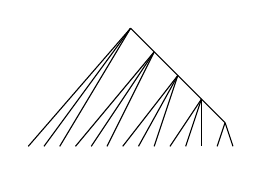
\begin{tikzpicture}[xscale=-0.2, yscale=0.3]
		\draw (1.5, 1) -- (1, 0);
		\draw (1.5, 1) -- (2, 0);
		\foreach \i in {2,...,5} {
			\draw ({\i*1.5}, \i) -- ({(\i-1)*1.5}, \i-1);
			\draw ({\i*1.5}, \i) -- ({3*(\i-1)}, 0);
			\draw ({\i*1.5}, \i) -- ({3*(\i-1)+1}, 0);
			\draw ({\i*1.5}, \i) -- ({3*(\i-1)+2}, 0);
		}
	\end{tikzpicture}
	\caption*{Overall Pattern}
\end{subfigure}

	\caption{Inner Node Structure for Sequential Insertions on an $m=4$ Tree}
	\label{fig:sequential-imbalance}
\end{figure}


\subsect{FPGA Implementation}

\begin{figure}
	\centering
	\begin{tikzpicture}[
	node distance = 0.5cm and 1cm,
	every node/.style={align=center, execute at begin node={\baselineskip=12pt}},
	mem/.style={draw, text width=4em},
	mod/.style={draw, text width=4em},
]
	% Modules
	\node[mem] (data-mem) {Data Memory};
	\node[mem, below=of data-mem] (req-mem) {Request Memory};
	\node[mem, below=of req-mem] (resp-mem) {Response Memory};
	\node[mod, right=of req-mem] (decoder) {Request Decoder};
	\node[mod, right=of resp-mem] (encoder) {Response Encoder};
	\node[mod, right=of decoder] (search) {Search Module};
	\node[mod, right=of encoder] (insert) {Insert Module};
	% Boundaries
	\draw[dashed] ($(data-mem.north west)+(-0.3,0.3)$)
		rectangle ($(resp-mem.south east)+(0.3,-0.3)$);
	\node[above=12pt of data-mem.north] {Shared with Host};
	% Connections
	\draw[->] (req-mem) -- (decoder);
	\draw[<-] (resp-mem) -- (encoder);
	\draw[->] ($(decoder.east)+(0,0.1)$) -- ($(search.west)+(0,0.1)$);
	\draw[->] ($(decoder.east)+(0,-0.1)$) -- ++(1em, 0)
		-- ($(insert.west)+(-1em,0.1)$) -- ++(1em, 0);
	\draw[<-] ($(encoder.east)+(0,0.1)$) -- ++(1em, 0)
		-- ($(search.west)+(-1em,-0.1)$) -- ++(1em, 0);
	\draw[<-] ($(encoder.east)+(0,-0.1)$) -- ($(insert.west)+(0,-0.1)$);
	\draw[->] ($(data-mem.east)+(0,-0.1)$) -| ($(search.east)+(0.4,0.0)$) -- ++(-0.4, 0);
	\draw[<->] ($(data-mem.east)+(0,0.1)$) -| ($(insert.east)+(0.6,0.0)$) -- ++(-0.6, 0);
\end{tikzpicture}

	\caption{Architecture of HLS Kernel}
	\label{fig:hls-arch}
\end{figure}

The FPGA's HLS implementation wraps a C implementation of the B-Link tree that
uses purely statically allocated memory. I/O between the host CPU system and the
FPGA is performed over PCIe using shared memory buffers. Separate buffers are
used for instructions and data memory, as this both simplifies access and gives
Vitis more flexibility to parallelize access to these buffers in order to
maximize memory bandwidth utility.

The compute kernel itself consists of four modules as shown in
\autoref{fig:hls-arch}; two handle I/O encoding/decoding and two handle tree
operations. Requests and responses are similar in structure to CPU operations; a
short opcode at the front delineates the operation and the remaining bits are
instruction specific, though care has been taken to align identical fields
shared between instructions so that they appear at the same offset. Operations
other than \texttt{NOP} return a status code indicating whether the operation
succeeded and the cause of its failure if applicable.

Though each search \& insert module can only handle one request at a time,
multiple copies of the kernel can be instantiated on the same FPGA, each of
which share the same host memory but with separate request/response buffers,
allowing for an analog to CPU multithreading.
